\documentclass{article}

\usepackage[dvipsnames]{xcolor}%barevne rozliseni kodu
\usepackage{mathptmx}
%packages for language
\usepackage[czech]{babel}
\usepackage[utf8]{inputenc}
%packages for graphic
\usepackage{graphicx}
\usepackage{pgfplots}
\usepackage{pgfplotstable}
\usepackage{multirow}
\usepackage{tikz}
\usepackage{import}
\usepackage[a4paper, total={17cm,25.7cm}, top=2cm, left=2cm, includefoot]{geometry}
\usepackage{todonotes}
\usepackage{standalone}
\usepackage{colortbl}%pro barevne zmeny v tabulce
\usepackage{float}
\usepackage{csvsimple} %pro import a práci s csv soubory
\usepackage{indentfirst}  % odsazení prvního řádku v odstavci
\usepackage{hyperref} %dela odkazy na mista v dokumentu atd
\usepackage{amsmath}%psani matic
\usepackage{mathrsfs}%psani kroucenym matematickym pismem
\usepackage{pdfpages}%vkladani celych pdf dokumentu
%cesta k obrazkum: ./Graphics/....
\usepackage{listings,lstautogobble}

\definecolor{mygreen}{rgb}{0,0.6,0}
\definecolor{mygray}{rgb}{0.5,0.5,0.5}
\definecolor{mymauve}{rgb}{0.58,0,0.82}

\lstset{language=Python,
	inputencoding=utf8,
	backgroundcolor=\color{white},   % choose the background color
	basicstyle=\footnotesize,        % size of fonts used for the code
	breaklines=true,                 % automatic line breaking only at whitespace
	captionpos=b,                    % sets the caption-position to bottom
	commentstyle=\color{mygray},    % comment style
	keywordstyle=\color{mymauve},       % keyword style
	stringstyle=\color{mygreen},     % string literal style
	numbers=left,
	extendedchars=true,
	literate= 
	{á}{{\'a}}1 
	{é}{{\'e}}1
	{ý}{{\'y}}1
	{í}{{\'i}}1 
	{ó}{{\'o}}1 
	{ú}{{\'u}}1
	{á}{{\'a}}1
	{í}{{\'i}}1
	{é}{{\'e}}1
	{ý}{{\'y}}1
	{ú}{{\'u}}1
	{ó}{{\'o}}1
	{ě}{{\v{e}}}1
	{š}{{\v{s}}}1
	{č}{{\v{c}}}1
	{ř}{{\v{r}}}1
	{ž}{{\v{z}}}1
	{ď}{{\v{d}}}1
	{ť}{{\v{t}}}1
	{ň}{{\v{n}}}1                
	{ů}{{\r{u}}}1
	{Á}{{\'A}}1
	{Í}{{\'I}}1
	{É}{{\'E}}1
	{Ý}{{\'Y}}1
	{Ú}{{\'U}}1
	{Ó}{{\'O}}1
	{Ě}{{\v{E}}}1
	{Š}{{\v{S}}}1
	{Č}{{\v{C}}}1
	{Ř}{{\v{R}}}1
	{Ž}{{\v{Z}}}1
	{Ď}{{\v{D}}}1
	{Ť}{{\v{T}}}1
	{Ň}{{\v{N}}}1                
	{Ů}{{\r{U}}}1
}

\begin{document}
	\begin{titlepage}
    \begin{center}
        \LARGE
        Západočeská Univerzita v Plzni\\
        Fakulta Aplikovaných Věd\\
        
        \vspace{1cm}
        
        
\includegraphics[width=0.5\textwidth]{./Graphics/FAV_logo.pdf}
        
        \vspace{4cm}
        
        \textbf{Bus Line Simulation}
        
        \vspace{0.5cm}
        Filip Jašek
        
    \end{center} 
    \vfill
        \noindent
        \large
        Předmět: KKY/MS1 (Modelování a simulace)\\
        Vyučující: Ing. Hajšman Václav, Ph.D., Ing. Liška Jindřich, Ph.D., Ing. Janeček Petr, Ph.D.\\
        Cvičící: Ing. Fetter Miloš\hfill Datum: \today
\end{titlepage}
	
	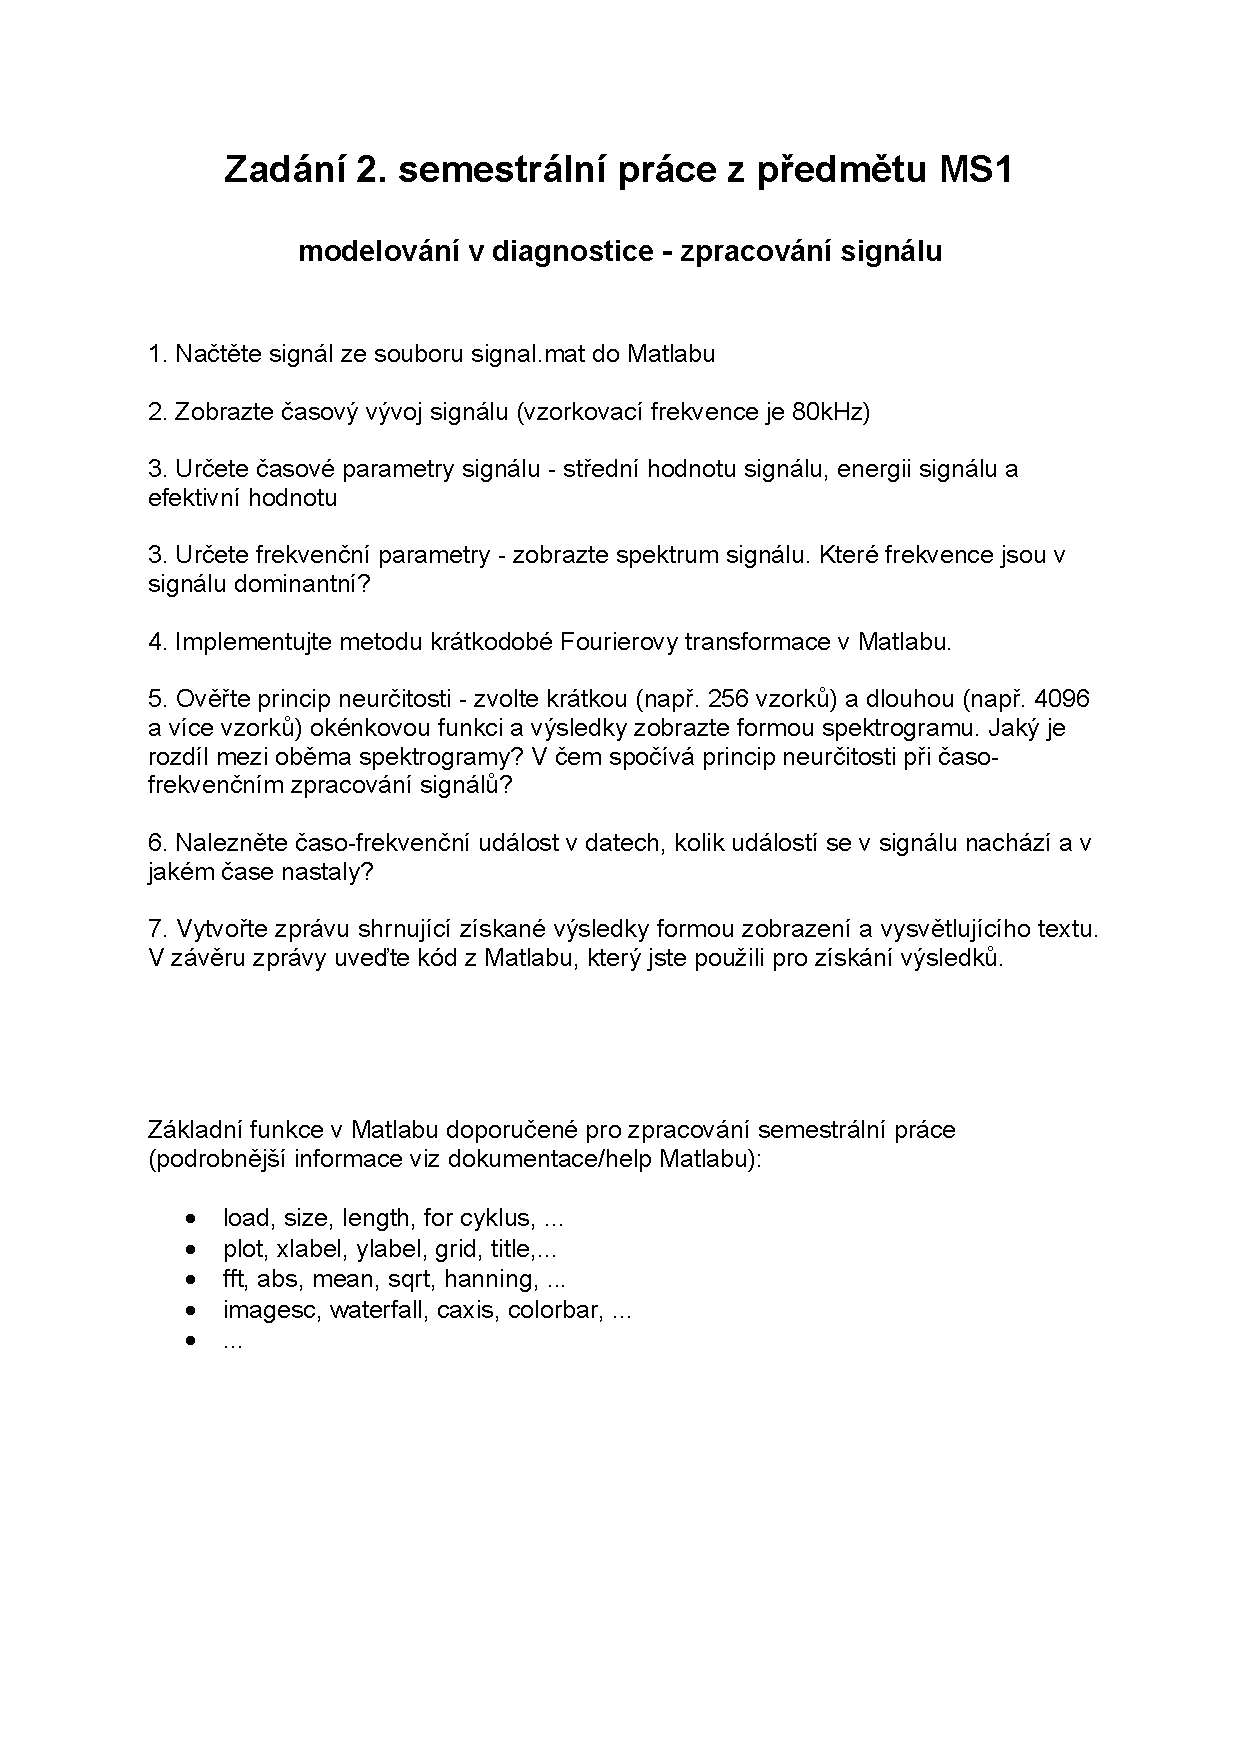
\includepdf[scale=.9,pages=1,pagecommand=\section{Zadání}]{./Graphics/MS1_semestralka02_zadani}
	\section{Vypracování}
		Samotné vypracování bylo provedeno v Pythonu za pomocí knihoven pandas, numpy a matplotlib. Tento přístup byl zvolen na základě faktu, že provedení v Pythonu umožňuje replikovat postup kýmkoliv bez ohledu na vlastnictví licence programu Matlab.
		\subsection{Načtení a zobrazení signálu}
			Z poskytnutého signálu ve formátu .mat byl extrahován signál do standardního csv souboru, který byl pak následně zpracován. Z poskytnuté informace o frekvenci \(f = 80kHz\) stanovíme periodu \(T = 1/f = 0.0000125 s\) a vytvoříme časovou osu s časovými přírůstky rovné periodě \(T\). Zjistíme tak, že vzorek signálu byl odebrán na časovém intervalu \(20s\). Průběh zadaného signálu v čase je zobrazen na následujícím obrázku \ref{graph:prubeh_signalu}. 
				\begin{figure}[H]
					\centering
					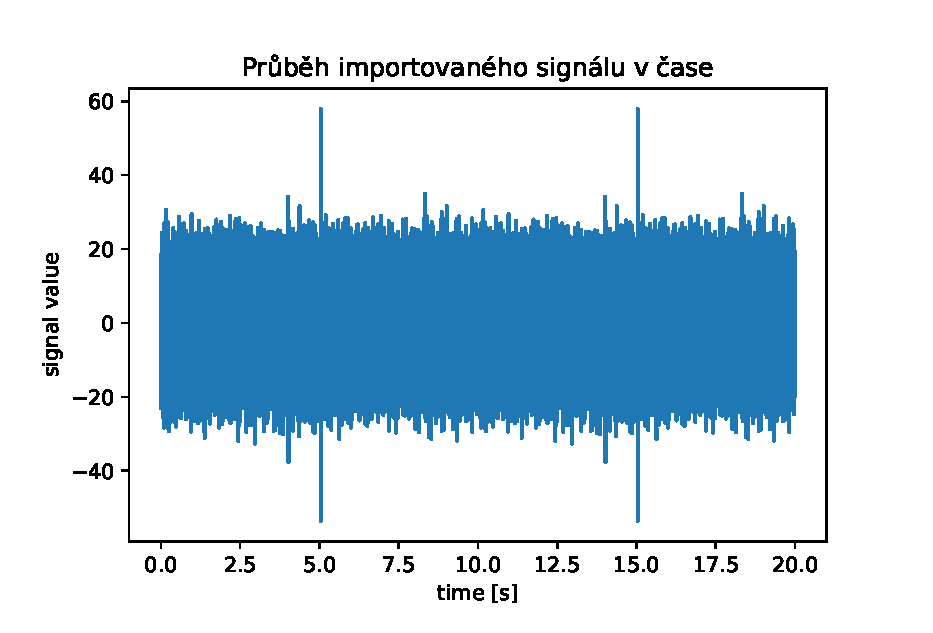
\includegraphics[width=\textwidth]{./Graphics/signal_v_case}
					\caption{Průběh zadaného signálu v čase.}
					\label{graph:prubeh_signalu}
				\end{figure}
			
		\subsection{Určení časových parametrů signálu}
			\noindent
			Střední hodnotu signálu určíme jako aritmetický průměr na konečném intervalu pomocí vzorce
			\[\overline{x} = \frac{1}{N}\cdot\sum_{t=0}^{N}x(t),\]
			kde \(\overline{x}\) je požadovaná střední hodnota, \(N=1600000\) je počet vzorků a \(x(t)\) hodnota signálu v časovém okamžiku \(t \in (0,N)\)\\
			
			\noindent
			Energii vypočteme za pomoci vektorového součinu samotného signálu se sebou a vydělením frekvencí  nebo použitím následujícího vzorce.
			\[E = T\cdot\sum_{t=0}^{N}x(t)^{2}\]
			Násobení periodou je nutné jelikož výpočet vychází ze spojitého vzorce
			\[E = \int_{-\infty}^{+\infty}|x(t)|^{2}dt,\]
			kde se počítá integrál z nekonečně malého přírůstku, zatímco pomocí sumy jen umocníme diskrétní časové okamžiky. Vynásobením periody tak stanovíme šířku jednotlivých obdélníků dané vzorkovací frekvencí \(f\).\\
			
			\noindent
			Výkon se pak dopočte jako
			\[P=\frac{1}{T\cdot N}\cdot E,\]
			jelikož je \(E\) již díky předchozímu výpočtu popsáno v závislosti na čase, je nutné podobně jako ve spojitém případě
			\[P = \lim_{X\to \infty} \frac{1}{2X} \int_{-X}^{+X}|x(t)|dt\]
			vydělit celkovým časem ve kterém byla energie spočtena.\\
			
			\noindent
			Efektivní hodnota je pak jednoduchá odmocnina vypočteného výkonu
			\[x_{ef} = \sqrt{P}.\]
			
			\noindent
			Pro zadaný signál vyšly následující výsledky:\\
			\verb|stredni hodnota signalu: -0.0003|\\
			\verb|energie signalu: 1025.6469|\\
			\verb|vykon signalu: 51.2823|\\
			\verb|efektivni hodnota signalu: 7.1612|\\
		
		\subsection{Určení frekvenčních parametrů}
			Pomocí absolutní hodnoty Fourierovy transformace byl získán symetrický graf spektra signálu od frekvence \(-40kHz\) do \(+40kHz\), který byl sečten do podoby v obrázku \ref{graph:spektrum_signalu} obsahující pouze kladné frekvence.\\
			
			\noindent
			V získaném grafu lze pozorovat, že dominantní frekvence jsou \(4798.2Hz\) a v okolí \(10kHz\).
				\begin{figure}[H]
					\centering
					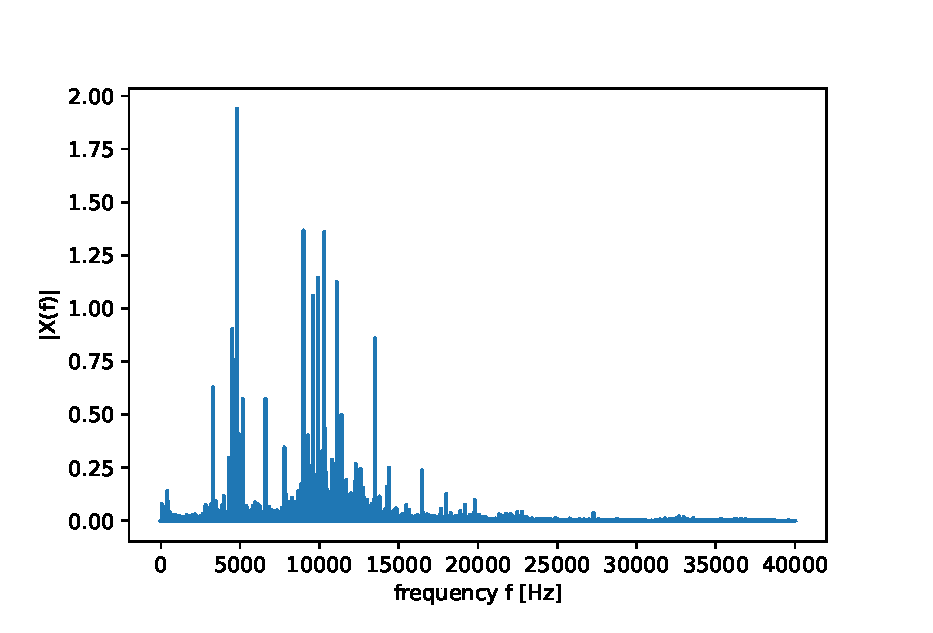
\includegraphics[width=\textwidth]{./Graphics/power_spectrum}
					\caption{Frekvenční spektrum zadaného signálu pro kladné frekvence.}
					\label{graph:spektrum_signalu}
				\end{figure}
		\subsection{Ověření principu neurčitosti}
			Princip neurčitosti spočívá v tom, že čím přesněji budeme chtít znát jednu vlastnost (zde signálu) tím nepřesněji budeme znát jinou. V našem případě zvětšováním okénkové funkce získáme přesnější informace o událostech v čase, ale na úkor přesnosti intenzit frekvencí. Při tvorbě spektrogramu počítáme s tím, že signál je na krátkém časovém okamžiku stacionární. Tento časový úsek definujeme pomocí velikosti okénka, na kterém se spočítá jedna průměrná hodnota podle typu okénka.\\
			
			\noindent
			Jak je ale z obrázku \ref{graph:okenkova_funkce} patrné, zvětšováním okénka jsme sice zvýraznili některé události v čase, ale zároveň ztratili jemnost měřítka ve frekvencích.\\
			
			\noindent
			Zde se dokonce podařilo větším okénkem \(2^{12}\) utlumit i jednu časovou událost v čase \(4s\). Pro potvrzení časových událostí jsem použil spektrogram vytvořený menším okénkem \(2^{8}\). Sečetl jsem hodnoty jednotlivých okénkách v čase a získal informaci, že signál obsahuje 4 časo-frekvenční události v časech 4, 5, 14 a 15s.
				\begin{figure}[H]
					\centering
					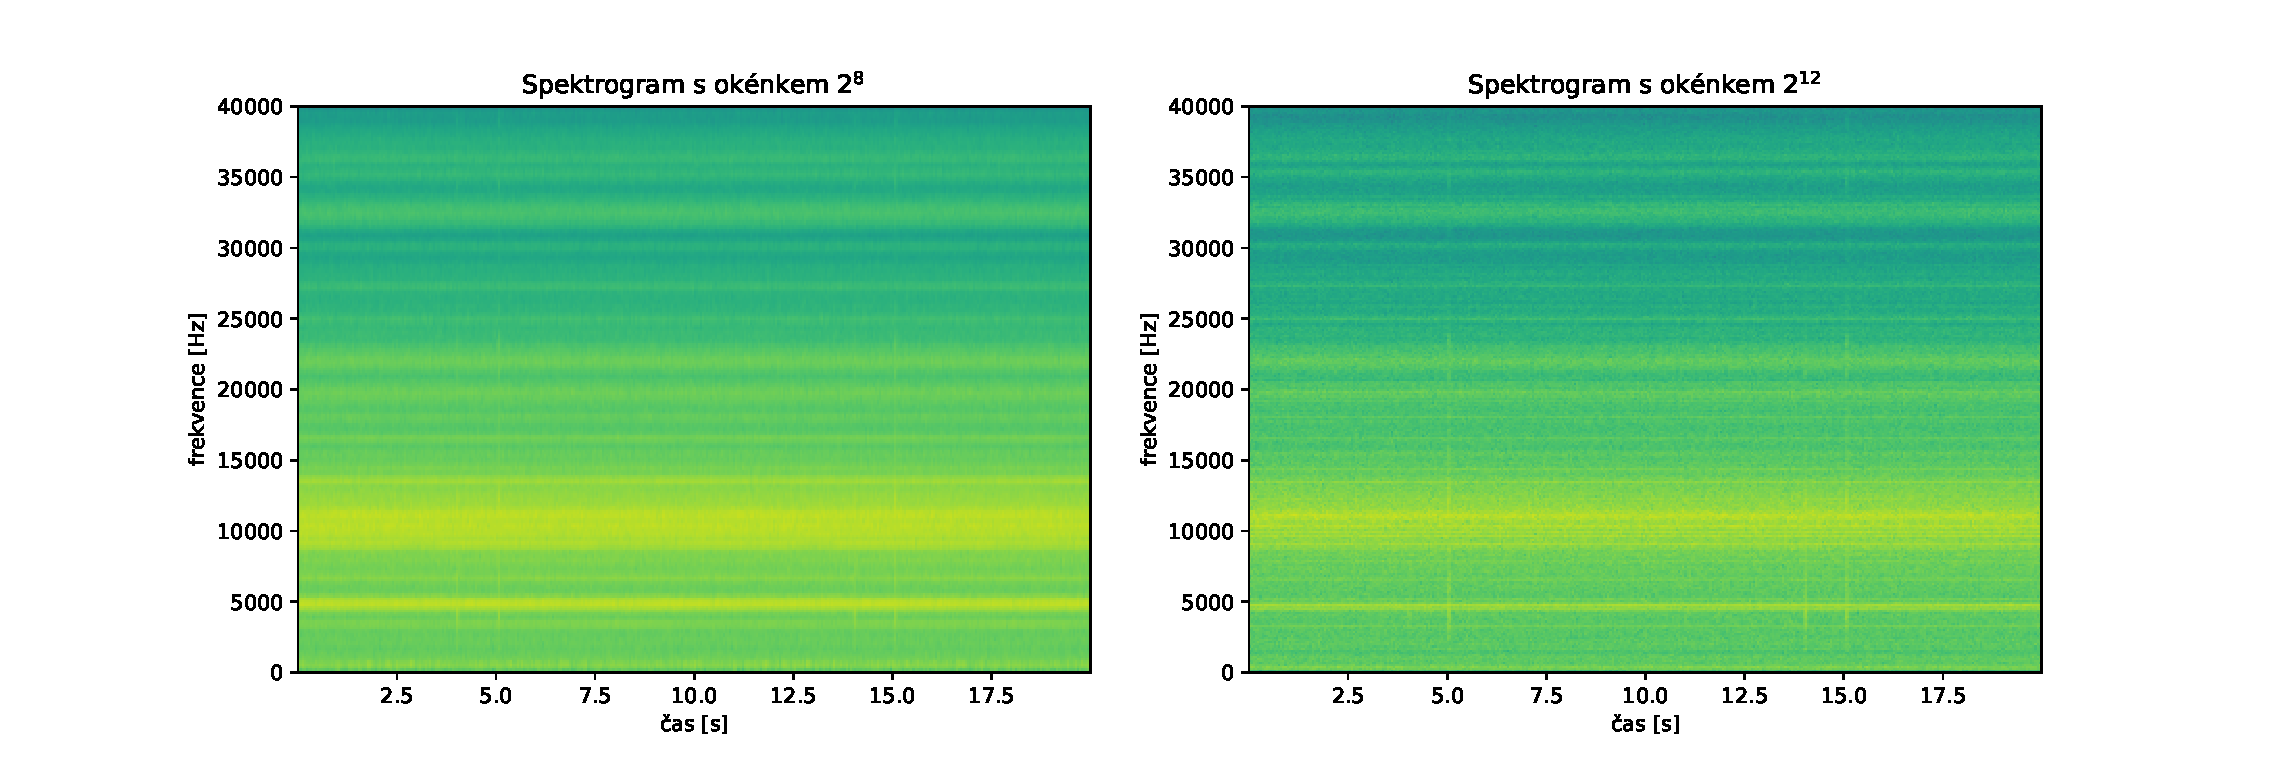
\includegraphics[width=\textwidth]{./Graphics/okenkova_funkce}
					\caption{Ověření principu neurčitosti za pomoci okénkové funkce.}
					\label{graph:okenkova_funkce}
				\end{figure}
	\newpage
	\section{Zdrojový kód}
		\lstinputlisting[inputencoding=utf8]{ms1_semestralka02.py}
	
\end{document}
